%
% $Id: figure.tex,v 1.1 2010/09/07 09:24:03 cvr Exp cvr $
% 
% 
\documentclass[a4paper]{article}
\usepackage[dvipsnames,svgnames]{xcolor}
\usepackage{tikz}
\usepackage{lfr}
\usetikzlibrary{shapes.gates.logic.US,trees,positioning,arrows}


\begin{document}

\begin{center}
\def\pgfont{\normalsize\color{black}\sffamily}
\def\vr{\vrule height6mm depth 4mm width0pt}

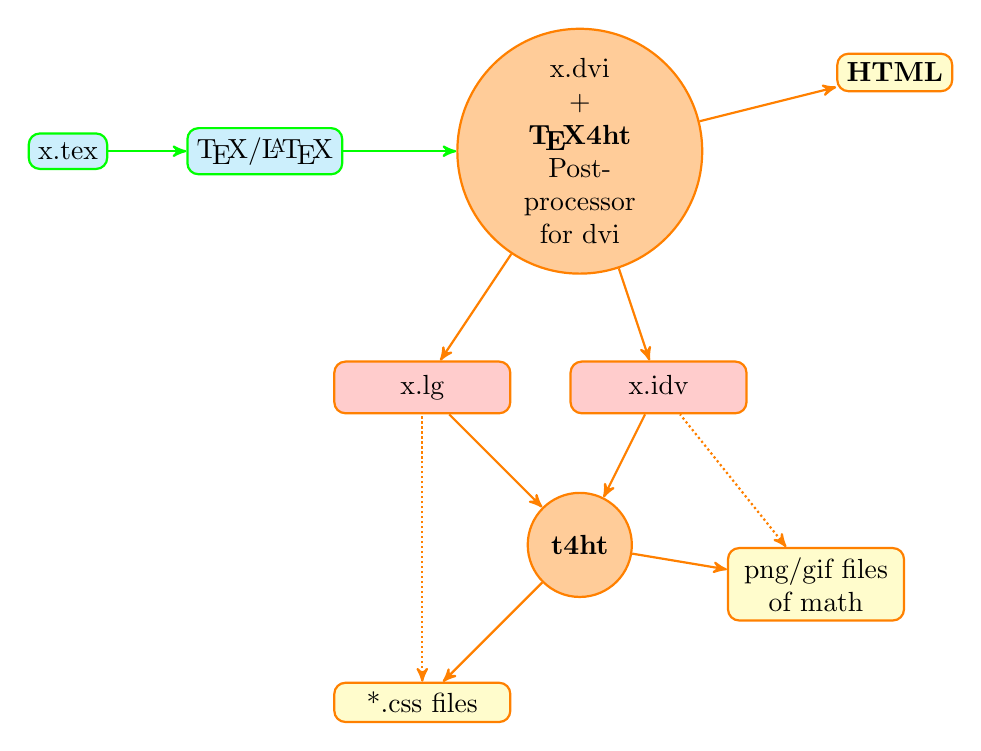
\begin{tikzpicture}
   \begin{scope}[xshift=-10cm,yshift=-5cm,thick,
                node distance=20mm,on grid,>=stealth',
    block/.style={font=\pgfont,rounded
       corners,rectangle,draw=green,fill=cyan!20},
    tex/.style={font=\pgfont,rounded
       corners,rectangle,draw=orange,fill=yellow!20},
    print/.style={font=\pgfont,text width=2cm,rounded
       corners,text centered,rectangle,draw=orange,fill=red!20},
    event/.style={rectangle,thick,draw=orange,fill=yellow!20,text width=2cm,
       text centered,font=\pgfont,anchor=north},
    be/.style={font=\pgfont,circle,thick,draw=orange,densely dotted,
       fill=yellow!10,anchor=north,minimum width=1.5cm},
    comp/.style={font=\pgfont,circle,draw=orange,fill=orange!40}]
   \node [comp]  (ca1)  
     {\parbox{15mm}{\centering x.dvi\\ $+$\\ {\bfseries\TeX4ht}\\
         Post-\\ processor\\ for dvi}};
   \node [tex]   (html) [right=of ca1,xshift=20mm,yshift=10mm]
     {\vr\bfseries HTML} edge [<-,draw=orange] (ca1) ;
   \node [print] (p1)   [below=of ca1,xshift=10mm,yshift=-10mm]
     {\strut x.idv} edge [<-,draw=orange] (ca1);
   \node [print] (e1) [below=of ca1,xshift=-20mm,yshift=-10mm]
     {\strut x.lg} edge [<-,draw=orange] (ca1);
   \node [block] (s2)   [left=of ca1,xshift=-20mm]
     {\vr\TeX/\LaTeX} edge [->,draw=green] (ca1);
   \node [block] (s1)   [left=of s2,xshift=-5mm]
     {x.tex} edge [->,draw=green] (s2);
   \node [comp]  (s4)   [below=of ca1,yshift=-30mm]
      {\parbox{10mm}{\centering\bfseries t4ht}} edge [<-,draw=orange] (p1)
         edge [<-,draw=orange] (e1) ;
   \node [tex]  (s5)   [left=of s4,yshift=-20mm]
      {\vr\parbox{20mm}{\centering*.css files}}
         edge [<-,draw=orange] (s4) edge [<-,densely dotted,draw=orange] (e1);
   \node [tex]  (s6)   [right=of s4,yshift=-5mm,xshift=10mm]
      {\vr\parbox{20mm}{\centering png/gif files \\ of math}}
         edge [<-,draw=orange] (s4) edge [<-,densely dotted,draw=orange] (p1);
  \end{scope}
\end{tikzpicture}
\end{center}

\end{document}